\apendice{Especificación de Requisitos}

\section{Introducción}
 
 Este apartado recoge los requisitos y objetivos del proyecto. Se detallarán los objetivos generales y tanto los requisitos funcionales como los no funcionales.

\section{Objetivos generales}

El principal objetivo de este proyecto es la creación de varias herramientas capaces de extraer y procesar información sobre un familia de productos concreta de Amazon, en este caso camisetas, para su posterior uso en estudios de mercado.

A su vez este proceso está divido en diferentes fases que podemos identificar como objetivos secundarios:

\begin{itemize}
	\item Extraer información de los distintos productos. Esta información incluye campos como el nombre de la marca, el rango de precios, número de valoraciones o imágenes del producto.
	\item Implementar un clasificador automático de imágenes.
	\item Almacenar la información descargada y las imágenes clasificadas en múltiples tablas con sus respectivos campos dentro de una base de datos.
	\item Visualizar la información descargada y procesada en un documento Excel.
\end{itemize}

\section{Catalogo de requisitos}

\subsection{Requisitos funcionales}
A continuación se muestran los requisitos funcionales que han sido implementados en las herramientas creadas para el proyecto:

\begin{itemize}
    \item \textbf{RF 1 Extraer información de los productos}. La herramienta debe ser capaz de extraer los diferentes campos de los productos deseados.
    \begin{itemize}
        \item \textbf{RF 1.1 Extraer los campos principales}. La aplicación debe ser capaz de extraer los campos principales de cada producto.
        \item \textbf{RF 1.2 Extraer las imágenes}. La aplicación debe de ser capaz de extraer los enlaces de las imágenes asociadas a cada producto.
        \item \textbf{RF 1.3 Extraer los comentarios}. La aplicación debe ser capaz de extraer los comentarios que los clientes han dejado a cada artículo.
    \end{itemize}
    %\item \textbf{RF 2 Lanzado por comando}. La herramienta debe de poder ser lanzada desde la linea de comandos.
    \item \textbf{RF 2 Almacenamiento en base de datos}. La herramienta debe ser capaz de almacenar la información extraída en una base de datos.
    \item \textbf{RF 3 Generar archivo JSON}. La aplicación debe ser capaz de generar un archivo JSON que contenga de forma estructurada todos los campos extraídos de cada producto.
    \begin{itemize}
        \item \textbf{RF 3.1 Generar un archivo JSON con los campos principales}. La herramienta debe ser capaz de generar un archivo JSON que contenga los campos principales de cada artículo y los enlaces a sus imágenes.
        \item \textbf{RF 3.2 Generar un archivo JSON con los comentarios}. La herramienta debe ser capaz de generar un archivo JSON que contenga los comentarios que los clientes han dejado a cada artículo.
    \end{itemize}
    \item \textbf{RF 4 Entrenar un clasificador de imágenes}. La herramienta debe poder entrenar un clasificador de imágenes.
    \begin{itemize}
        \item \textbf{RF 4.1 Conjunto de entrenamiento}. La herramienta ha de ser capaz de crear un conjunto de datos de entrenamiento para entrenar los clasificadores.
        \item \textbf{RF 4.2 Entrenar clasificador modelos}. La herramienta debe de ser capaz de entrenar un clasificador de imágenes que detecte si en una imagen aparece un modelo o no.
        \item \textbf{RF 4.3 Entrenar clasificador caras}. La herramienta debe ser capaz de entrenar un clasificador de imágenes que detecte si en una imagen la cara de un modelo es visible o no.
    \end{itemize}
    \item \textbf{RF 5 Clasificar automáticamente imágenes}. La herramienta ha de ser capaz de clasificar imágenes de forma automática.
    \begin{itemize}
        \item \textbf{RF 5.1 Clasificador modelos}. La herramienta debe ser capaz de clasificar imágenes en función de si en una imagen aparece un modelo o no.
        \item \textbf{RF 5.2 Clasificador caras}. La herramienta debe ser capaz de clasificar imágenes en función de si en una imagen la cara de un modelo es visible o no.
    \end{itemize}
    \item \textbf{RF 6 Generar Excel}. La herramienta ha de ser capaz de generar un documento Excel que contenga toda la información sobre los productos extraídos, a partir de la base de datos existente. 
    
\end{itemize}

\subsection{Requisitos no funcionales}

\begin{itemize}
    \item \textbf{RNF 1 Proceso automático}. Todo el proceso, desde la extracción de datos a la generación del documento final, ha de ser lo mas automatizado posible.
    \item \textbf{RNF 2 Facilidad instalación}. La herramienta debe ser fácil de instalar y ponerse en marcha.
    \item \textbf{RNF 2 Software libre}. La herramienta ha de utilizar software libre.
\end{itemize}

\section{Especificación de requisitos}

\subsection{Diagramas de casos de  uso}

Los siguientes diagramas muestran los casos de uso de los requisitos definidos previamente. Han sido creados con la herramienta Creately\footnote{\url{https://app.creately.com}}.

\FloatBarrier
\begin{figure}[!h]
\centering
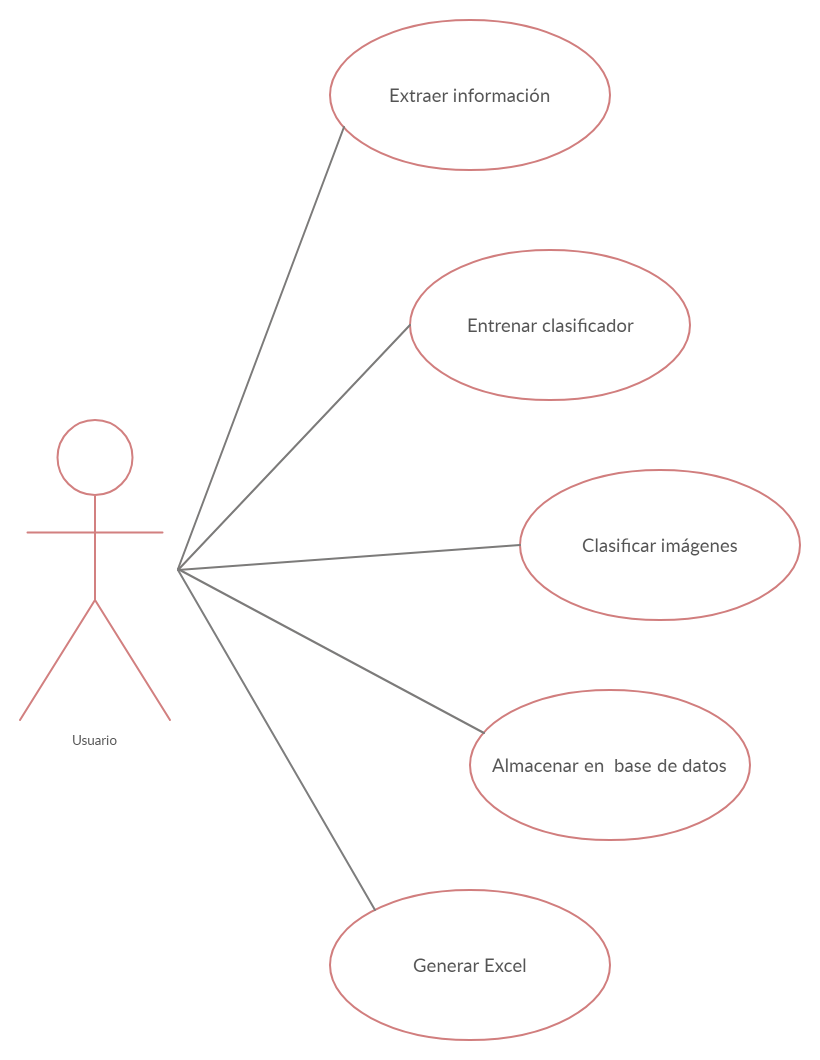
\includegraphics[width=0.6\textwidth]{anexos/caso_uso1}
\caption[Diagrama general de los casos de uso]{Diagrama general de los casos de uso}
\label{fig:caso}
\end{figure}
\FloatBarrier
%\imagen{anexos/caso_uso1}{Diagrama general de los casos de uso}

\FloatBarrier
\begin{figure}[!h]
\centering
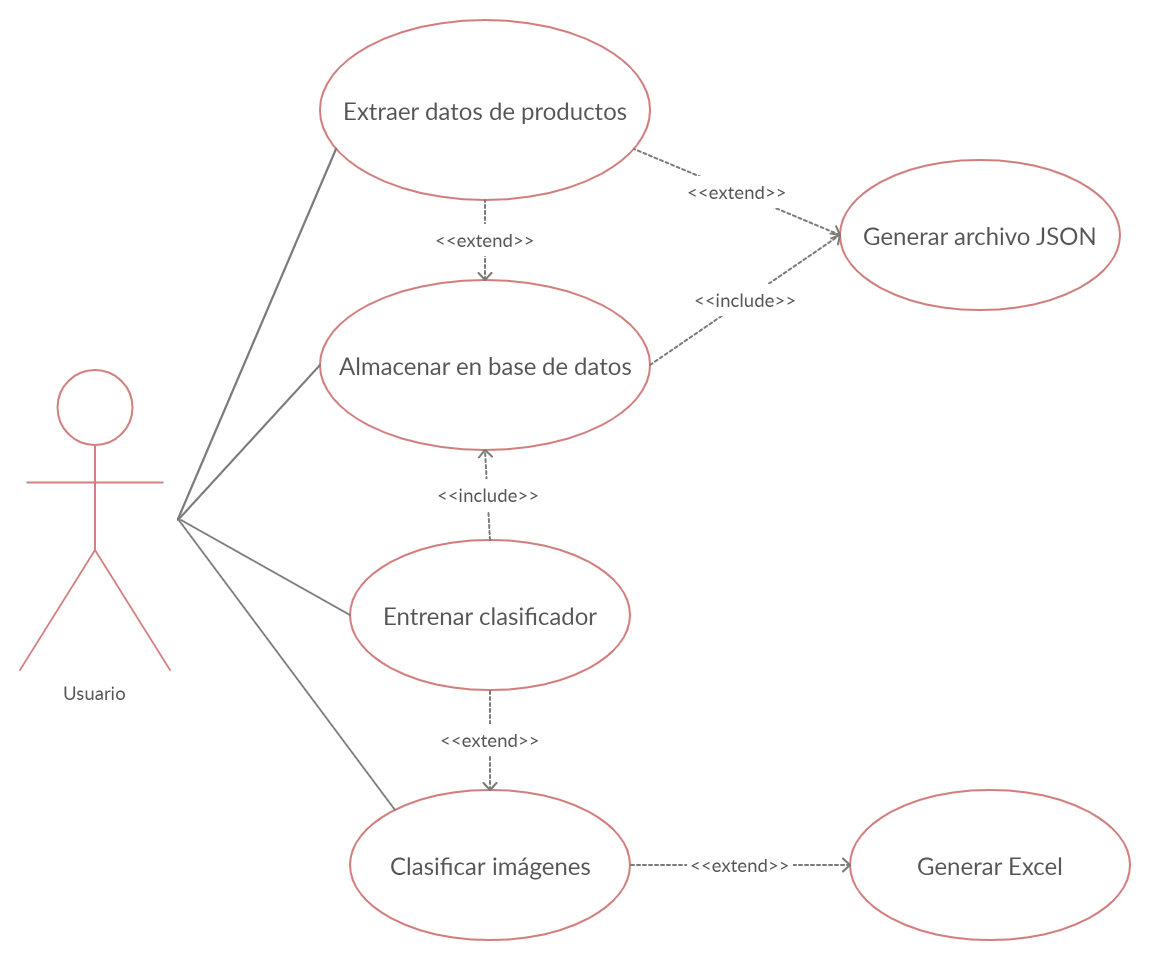
\includegraphics[width=0.7\textwidth]{anexos/caso_uso2}
\caption[Diagrama desglosado de los casos de uso del usuario]{Diagrama desglosado de los casos de uso del usuario}
\label{fig:caso}
\end{figure}
\FloatBarrier
%\imagen{anexos/caso_uso2}{Diagrama desglosado de los casos de uso del usuario}

%CASO DE USO 1

\tablaSmallSinColores{Caso de uso 1: Extraer información de los productos.}{p{3cm} p{.75cm} p{9.5cm}}{tablaUC1}{
  \multicolumn{3}{l}{Caso de uso 1: Extraer información de los productos.} \\
 }
 {
  Descripción                            & \multicolumn{2}{p{10.25cm}}{Permite al usuario extraer la información los productos deseados.} \\\hline
  \multirow{2}{3.5cm}{Requisitos}   &\multicolumn{2}{p{10.25cm}}{RF 1} \\\cline{2-3}
                                         & \multicolumn{2}{p{10.25cm}}{RF 1.1} \\\cline{2-3}
                                         & \multicolumn{2}{p{10.25cm}}{RF 1.2} \\\cline{2-3}
                                         & \multicolumn{2}{p{10.25cm}}{RF 1.3} 
                                         \\\hline
  Precondiciones                         &  \multicolumn{2}{p{10.25cm}}{Es necesaria conexión a Internet y los enlaces de los productos a extraer.}   \\\hline
  \multirow{2}{3.5cm}{Secuencia normal}  & Paso & Acción \\\cline{2-3}
                                         & 1    & El usuario indica el fichero que contiene los enlaces de los productos.
  \\\cline{2-3}
                                         & 2    & Se inicia el proceso de \english{web scraping}.
  \\\cline{2-3}
                                         & 3    & Se extrae de forma secuencial todos los campos de todos los productos seleccionados.
    \\\cline{2-3}
                                         & 4    & Se guarda en la base de datos la información extraída. 
                                         \\\hline
  Postcondiciones                        & \multicolumn{2}{p{10.25cm}}{Se ha extraído y almacenado la información de los productos deseados.} \\\hline
  Excepciones                        & \multicolumn{2}{p{10.25cm}}{No se ha podido acceder a <<Amazon.com>>.}\\\hline
  Importancia                            & Alta \\\hline
  Urgencia                               & Alta \\
}

%CASO DE USO 2

%\tablaSmallSinColores{Caso de uso 2: Lanzado  por  comando.}{p{3cm} p{.75cm} p{9.5cm}}{tablaUC1}{
%  \multicolumn{3}{l}{Caso de uso 2: Lanzado  por  comando.} \\
% }
% {
%  Descripción                            & \multicolumn{2}{p{10.25cm}}{Permite al usuario lanzar por comando la herramienta de \english{web %scrpaing}.} \\\hline
%  \multirow{2}{3.5cm}{Requisitos}   &\multicolumn{2}{p{10.25cm}}{RF 1} \\\cline{2-3}
%                                         & \multicolumn{2}{p{10.25cm}}{RF 2}
%                                         \\\hline
%  Precondiciones                         &  \multicolumn{2}{p{10.25cm}}{Es necesario disponer de una terminal o consola de comandos y conocer la ruta donde se encuentra el proyecto.}   \\\hline
%  \multirow{2}{3.5cm}{Secuencia normal}  & Paso & Acción \\\cline{2-3}
%                                         & 1    & El usuario ha de escribir el comando y el nombre del \english{spider} junto con el nombre del fichero JSON donde se almacenará la información.
%  \\\cline{2-3}
%                                         & 2    & Se lanza el comando para iniciar el proceso. 
%                                         \\\hline
%  Postcondiciones                        & \multicolumn{2}{p{10.25cm}}{Comienza correctamente el proceso de extracción de datos.} \\\hline
%  Excepciones                        & \multicolumn{2}{p{10.25cm}}{Sintaxis incorrecto.}\\\hline
%  Importancia                            & Baja \\\hline
%  Urgencia                               & Baja \\
%}



%CASO DE USO 3

\tablaSmallSinColores{Caso de uso 2: Almacenamiento en base de datos.}{p{3cm} p{.75cm} p{9.5cm}}{tablaUC1}{
  \multicolumn{3}{l}{Caso de uso 2: Almacenamiento en base de datos.} \\
 }
 {
  Descripción                            & \multicolumn{2}{p{10.25cm}}{Permite al usuario almacenar la información extraída en una base de datos.} \\\hline
  \multirow{2}{3.5cm}{Requisitos}   &\multicolumn{2}{p{10.25cm}}{RF 1} \\\cline{2-3}
                                         & \multicolumn{2}{p{10.25cm}}{RF 2} 
                                         \\\hline
  Precondiciones                         &  \multicolumn{2}{p{10.25cm}}{Se debe haber ejecutado el \english{web scraper}.}   \\\hline
  \multirow{2}{3.5cm}{Secuencia normal}  & Paso & Acción \\\cline{2-3}
                                         & 1    & Se crea una conexión con la base de datos.
  \\\cline{2-3}
                                         & 2    & Se crean las diferentes tablas y sus campos.
  \\\cline{2-3}
                                         & 3    & Se almacenan los campos de los productos descargados.
    \\\cline{2-3}
                                         & 4    & Se cierra la conexión con la base de datos
                                         \\\hline
  Postcondiciones                        & \multicolumn{2}{p{10.25cm}}{Todos los campos quedan almacenados correctamente.} \\\hline
  Excepciones                        & \multicolumn{2}{p{10.25cm}}{Excepción SQL o sintaxis incorrecto.}\\\hline
  Importancia                            & Alta \\\hline
  Urgencia                               & Media \\
}


%CASO DE USO 4

\tablaSmallSinColores{Caso de uso 3: Generar archivo JSON.}{p{3cm} p{.75cm} p{9.5cm}}{tablaUC1}{
  \multicolumn{3}{l}{Caso de uso 3: Generar archivo JSON.} \\
 }
 {
  Descripción                            & \multicolumn{2}{p{10.25cm}}{Permite al usuario extraer la información los productos deseados.} \\\hline
  \multirow{2}{3.5cm}{Requisitos}   &\multicolumn{2}{p{10.25cm}}{RF 1} \\\cline{2-3}
                                         & \multicolumn{2}{p{10.25cm}}{RF 2}
                                         \\\hline
  Precondiciones                         &  \multicolumn{2}{p{10.25cm}}{Es necesario disponer de una terminal y conocer la ruta donde se desea guardar el archivo JSON.}   \\\hline
  \multirow{2}{3.5cm}{Secuencia normal}  & Paso & Acción \\\cline{2-3}
                                         & 1    & El usuario indica la ruta del archivo que desea crear.
  \\\cline{2-3}
                                         & 2    & Se inicia el proceso de \english{web scraping}.
                                         \\\hline
  Postcondiciones                        & \multicolumn{2}{p{10.25cm}}{Se genera correctamente el fichero JSON que contiene la información descargada.} \\\hline
  Excepciones                        & \multicolumn{2}{p{10.25cm}}{Error de sintaxis.}\\\hline
  Importancia                            & Media \\\hline
  Urgencia                               & Media \\
}

%CASO DE USO 5

\tablaSmallSinColores{Caso de uso 4: Entrenar un clasificador de imágenes.}{p{3cm} p{.75cm} p{9.5cm}}{tablaUC1}{
  \multicolumn{3}{l}{Caso de uso 4: Entrenar un clasificador de imágenes.} \\
 }
 {
  Descripción                            & \multicolumn{2}{p{10.25cm}}{Permite al usuario extraer la información los productos deseados.} \\\hline
  \multirow{2}{3.5cm}{Requisitos}   &\multicolumn{2}{p{10.25cm}}{RF 1} \\\cline{2-3}
                                         & \multicolumn{2}{p{10.25cm}}{RF 1.1} \\\cline{2-3}
                                         & \multicolumn{2}{p{10.25cm}}{RF 1.2} \\\cline{2-3}
                                         & \multicolumn{2}{p{10.25cm}}{RF 1.3} 
                                         \\\hline
  Precondiciones                         &  \multicolumn{2}{p{10.25cm}}{Es necesario disponer del conjunto de datos de entrenamiento.}   \\\hline
  \multirow{2}{3.5cm}{Secuencia normal}  & Paso & Acción \\\cline{2-3}
                                         & 1    & Se descargan las imágenes etiquetadas manualmente.
  \\\cline{2-3}
                                         & 2    & Se divide el conjunto en 2 subconjuntos: entrenamiento y test.
  \\\cline{2-3}
                                         & 3    & Se comienza a entrenar el clasificador a partir de estos conjuntos.
    \\\cline{2-3}
                                         & 4    & Se descarga el clasificador ya entrenado para su posterior uso. 
                                         \\\hline
  Postcondiciones                        & \multicolumn{2}{p{10.25cm}}{Se entrenado correctamente el clasificador y es capaz de etiquetar las imágenes con un a precisión aceptable.} \\\hline
  Excepciones                        & \multicolumn{2}{p{10.25cm}}{Error de sintaxis.}\\\hline
  Importancia                            & Alta \\\hline
  Urgencia                               & Alta \\
}

%CASO DE USO 6

\tablaSmallSinColores{Caso de uso 5: Clasificar automáticamente las imágenes.}{p{3cm} p{.75cm} p{9.5cm}}{tablaUC1}{
  \multicolumn{3}{l}{Caso de uso 5: Clasificar automáticamente las imágenes.} \\
 }
 {
  Descripción                            & \multicolumn{2}{p{10.25cm}}{Permite al usuario extraer la información los productos deseados.} \\\hline
  \multirow{2}{3.5cm}{Requisitos}   &\multicolumn{2}{p{10.25cm}}{RF 1} \\\cline{2-3}
                                         & \multicolumn{2}{p{10.25cm}}{RF 1.1} \\\cline{2-3}
                                         & \multicolumn{2}{p{10.25cm}}{RF 1.2} \\\cline{2-3}
                                         & \multicolumn{2}{p{10.25cm}}{RF 1.3} \\\cline{2-3}
                                         & \multicolumn{2}{p{10.25cm}}{RF 3.1} \\\cline{2-3}
                                         & \multicolumn{2}{p{10.25cm}}{RF 4} \\\cline{2-3}
                                         & \multicolumn{2}{p{10.25cm}}{RF 4.1} \\\cline{2-3}
                                         & \multicolumn{2}{p{10.25cm}}{RF 4.2} \\\cline{2-3}
                                         & \multicolumn{2}{p{10.25cm}}{RF 4.3} 
                                         \\\hline
  Precondiciones                         &  \multicolumn{2}{p{10.25cm}}{Es necesario disponer de un  clasificador previamente entrenado.}   \\\hline
  \multirow{2}{3.5cm}{Secuencia normal}  & Paso & Acción \\\cline{2-3}
                                         & 1    & El usuario indica la ruta de los productos de los que desea clasificar sus imágenes.
  \\\cline{2-3}
                                         & 2    & El clasificador itera sobre estas imágenes anotando una etiqueta en cada una en función de su clasificación.
  \\\cline{2-3}
                                         & 4    & Se guardan en la base de datos las anotaciones generadas asociadas a cada producto. 
                                         \\\hline
  Postcondiciones                        & \multicolumn{2}{p{10.25cm}}{Las imágenes han sido clasificadas y las anotaciones almacenadas.} \\\hline
  Excepciones                        & \multicolumn{2}{p{10.25cm}}{Error de sintaxis. Error al cargar una imagen. Error al clasificar. Excepción SQL}\\\hline
  Importancia                            & Alta \\\hline
  Urgencia                               & Alta \\
}

%CASO DE USO 7

\tablaSmallSinColores{Caso de uso 6: Generar documento Excel.}{p{3cm} p{.75cm} p{9.5cm}}{tablaUC1}{
  \multicolumn{3}{l}{Caso de uso 6: Generar documento Excel.} \\
 }
 {
  Descripción                            & \multicolumn{2}{p{10.25cm}}{Permite al usuario generar un documento Excel con toda la información descargada y procesada.} \\\hline
  \multirow{2}{3.5cm}{Requisitos}   &\multicolumn{2}{p{10.25cm}}{RF 1} \\\cline{2-3}
                                         & \multicolumn{2}{p{10.25cm}}{RF 1.1} \\\cline{2-3}
                                         & \multicolumn{2}{p{10.25cm}}{RF 1.2} \\\cline{2-3}
                                         & \multicolumn{2}{p{10.25cm}}{RF 1.3} \\\cline{2-3}
                                         & \multicolumn{2}{p{10.25cm}}{RF 3.1} \\\cline{2-3}
                                         & \multicolumn{2}{p{10.25cm}}{RF 4} \\\cline{2-3}
                                         & \multicolumn{2}{p{10.25cm}}{RF 4.1} \\\cline{2-3}
                                         & \multicolumn{2}{p{10.25cm}}{RF 4.2} \\\cline{2-3}
                                         & \multicolumn{2}{p{10.25cm}}{RF 4.3} 
                                         \\\hline
  Precondiciones                         &  \multicolumn{2}{p{10.25cm}}{Es necesario disponer de la base de datos completa junto con las predicciones del clasificador de imágenes.}   \\\hline
  \multirow{2}{3.5cm}{Secuencia normal}  & Paso & Acción \\\cline{2-3}
                                         & 1    & Creación de \english{dataframes} con la ayuda de la librería Pandas a partir de la base de datos.
  \\\cline{2-3}
                                         & 2    & Generación del documento Excel a partir de los \english{dataframes} creados anteriormente.
  \\\cline{2-3}
                                         & 4    & Descarga del documento Excel que contiene toda la información. 
                                         \\\hline
  Postcondiciones                        & \multicolumn{2}{p{10.25cm}}{Se ha generado un documento excel con la información de cada producto y la predicción que ha devuelto el clasificador de imágenes.} \\\hline
  Excepciones                        & \multicolumn{2}{p{10.25cm}}{Error de sintaxis. Error al conectar con la base de datos.}\\\hline
  Importancia                            & Alta \\\hline
  Urgencia                               & Alta \\
}